\documentclass[11pt]{article}
\usepackage[fleqn]{amsmath}\textwidth 6.5in
\oddsidemargin -0.25in
%\evensidemargin -0.5in
\topmargin -0.25in
\textheight 9.0in

\newcommand{\docname}{\bf wvs-048r7}
\newcommand{\docdate}{29 April 2009}

\usepackage{graphicx}

\usepackage{floatflt}

\begin{document}

%\tracingcommands=1
\newlength{\hW} % heading box width
\newlength{\pW} % page number field width
\settowidth{\hW}{\docname}
\settowidth{\pW}{Page \pageref{lastpage}\ of \pageref{lastpage}}
\ifdim \pW > \hW \setlength{\hW}{\pW} \fi
\makeatletter
\def\@biblabel#1{#1.}
\newcommand{\ps@twolines}{%
  \renewcommand{\@oddhead}{%
    \docdate\hfill\parbox[t]{\hW}{{\hfill\docname}\newline
                          Page \thepage\ of \pageref{lastpage}}}%
\renewcommand{\@evenhead}{}%
\renewcommand{\@oddfoot}{}%
\renewcommand{\@evenfoot}{}%
}%
\makeatother
\pagestyle{twolines}

\vspace{-10pt}
\begin{tabbing}
\phantom{References: }\= \\
To: \>Bill\\
Subject: \>Different solution for $\phi$--$H$ calculation in {\tt metrics\_m}\\
From: \>Van Snyder\\
\end{tabbing}

\parindent 0pt \parskip 10pt
\vspace{-20pt}

\newcommand\Req{R^\oplus_{\text{eq}}}

\begin{floatingfigure}{3.75in}
{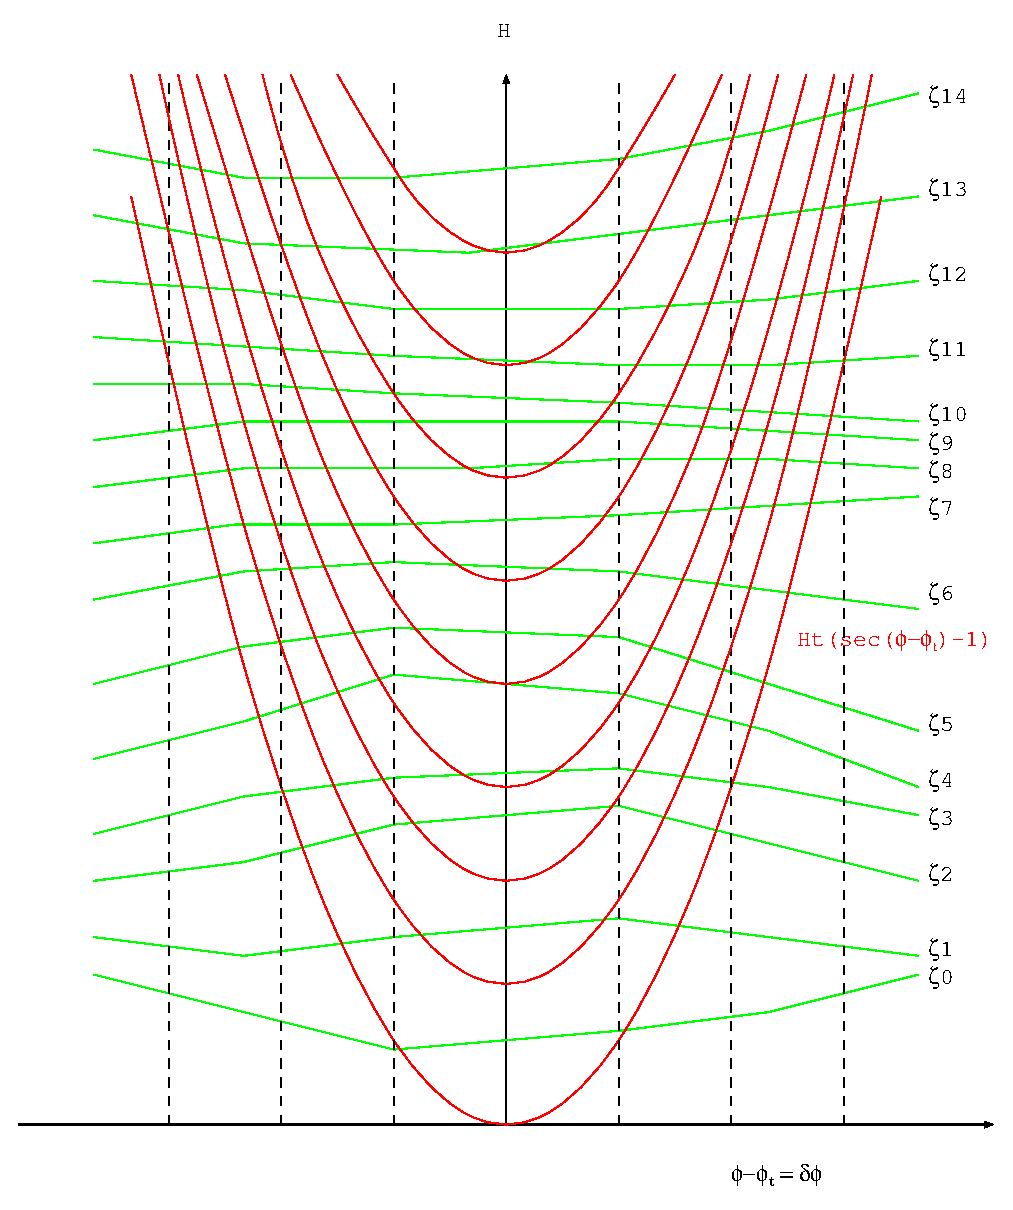
\includegraphics[width=3.5in,height=4.5in,clip]{./wvs-048-grid2.eps}}
\end{floatingfigure}

We want to solve for $\phi$ and $H$ at the intersections of the line of
sight with constant-$\zeta$ surfaces.

Normally one thinks of the line of sight as a straight line, and
constant-$\zeta$ surfaces as approximate circles roughly concentric with
the earth.

This diagram shows the line of sight intersecting the constant-$\zeta$
surfaces in cartesian $\phi$--$H$ co\"{o}rdinates instead of polar 
$\phi$--$\zeta$ co\"{o}rdinates.  The con\-stant-$\zeta$ surfaces are the
green lines, the lines of sight are the red lines, and the temperature
$\phi$ basis $\phi_1 \dots \phi_n$ is the vertical black lines.  The
quantity $H-\Req$, where $\Req$ is the equivalent circular earth radius,
is given at specified values of $\phi$ and $\zeta$, i.e. at the
intersections of the green and black lines, by the array {\tt H\_ref}. 
The tangent height $H_t$, $\Req$, and $\phi_1 \dots \phi_n$ are given.

Denote {\tt H\_ref} by $H_{ij}$.  Each row of {\tt H\_ref} gives the
endpoints of a piecewise-linear con\-stant-$\zeta$ surface.  Writing the
intersection of that line with the line of sight expressed as a function
of $\phi$, \emph{viz.} $H = H_t \sec \phi$, interpolating $H$ linearly in
$\phi$ between $H_{ij}$ and $H_{i,j+1}$, using $H_\text{tan} = H_t -
\Req$, and subtracting $H_t$ from both sides to cancel $\Req$ on the left
side, we need to solve

\begin{equation}\begin{split}\label{one}
H_{ij} + \Req + (H_{i,j+1}-H_{ij})
                  \frac{\phi-\phi_j}
                       {\phi_{j+1}-\phi_j} -
                  ( H_\text{tan} + \Req ) \,&= \\
H_{ij} + (H_{i,j+1}-H_{ij})
                  \frac{\phi-\phi_j}
                       {\phi_{j+1}-\phi_j} -
                  H_\text{tan} \,&= \\
H_{ij} + (H_{i,j+1}-H_{ij})
                  \frac{(\phi-\phi_t)-(\phi_j-\phi_t)}
                       {\phi_{j+1}-\phi_j} -
                  H_\text{tan} \,&=
H_t(\sec ( \phi - \phi_t ) - 1) \\
\end{split}\end{equation}

when $\phi_1 \leq \phi \leq \phi_n$, where $n$ is the number of columns
in {\tt H\_ref}, for all $i$ and $j$.  For $\phi < \phi_1$ or $\phi >
\phi_n$ assume constant-$\zeta$ surfaces are also constant-$H$ surfaces,
i.e., $H_{i0} = H_{i1}$ and $H_{in} = H_{i,n+1}$, which reduces the above
to $H_{i0} = H_t \sec(\phi-\phi_t)$ or $H_{in} = H_t \sec(\phi-\phi_t)$.

We write Equation (\ref{one}) as a zero-finding problem

\begin{equation}\label{two}
d(\delta\phi) = a\, (\sec\delta\phi-1) + b\, \delta\phi + c = 0
\end{equation}

where

\begin{equation}\begin{split}
\delta\phi =\,& \phi - \phi_t\,, \\
a =\,& (\phi_{j+1}-\phi_j) H_t\,, \\
b =\,& -(H_{i,j+1}-H_{ij})\,, \text{ and} \\
c =\,& - H_{ij} (\phi_{j+1}-\phi_t) + H_{i,j+1} (\phi_j-\phi_t) +
(\phi_{j+1}-\phi_j) H_\text{tan} \,.\\
\end{split}\end{equation}

To start a Newton iteration to solve Equation(\ref{two}), use
$\sec\delta\phi \approx 1 + \frac12 \delta\phi^2$, and solve for
$\delta\phi$ in

\begin{equation}
 \frac12 a\, \delta\phi^2 + b \, \delta\phi + c = 0\,.
\end{equation}

To the left of the tangent point, choose the minimum of the two
solutions; otherwise, choose the maximum.  This potentially has two
solutions at the tangent point unless the tangent point is at one of the
reference $\zeta$ values.  The existing code forces $\delta\phi$ to be
zero at the tangent.

When $\delta\phi < 0.2$ radians use an $8^\text{th}$-order polynomial

\begin{equation}
\sec\delta\phi - 1 \approx P_8(\delta\phi) =
 \frac12 \delta\phi^2 + \frac5{24} \delta\phi^4
 + \frac{61}{720} \delta\phi^6 + \frac{277}{8064} \delta\phi^8
\end{equation}

to approximate $\sec \delta \phi -1$ because the latter suffers
cancellation when $\delta\phi \approx 0$, giving

\begin{equation}
a\, P_8(\delta\phi) + b\, \delta\phi + c \approx 0\,.
\end{equation}

Using 16-digit arithmetic, $-1.5 \times 10^{-9} < P_8(\delta\phi) -
\sec(\delta\phi) + 1 \leq 0$ for $|\delta\phi| \leq 0.2$.

For the Newton iteration $\delta\phi_{n+1} = \delta\phi_n - d(\delta\phi) /
d^\prime(\delta\phi)$ the derivatives

\begin{equation}
d^\prime(\delta\phi) = a\, \sec \delta\phi \tan \delta\phi + b \approx
 P_8^\prime(\delta\phi) + b
\end{equation}

are necessary.  Remember, $\tan\delta\phi = \text{signum}(\delta\phi)
\sqrt{\sec^2 \delta\phi - 1}$, not simply $\sqrt{\sec^2 \delta\phi - 1}$.

\label{lastpage}
\end{document}
% $Id$

% $Log$
% Revision 1.6  2009/04/30 02:40:29  vsnyder
% Correct a sign error, derivatives
%
% Revision 1.5  2009/04/29 22:35:08  vsnyder
% Clarify and simplify
%
% Revision 1.4  2009/04/28 02:55:18  vsnyder
% Make notation more consistent
%
% Revision 1.3  2009/04/28 00:41:58  vsnyder
% Undo erroneous sign change - wvs-048r2 is correct
%
